\documentclass{protokol}
\usepackage{graphicx}
\usepackage{float}

\usepackage{tikz}
\usetikzlibrary{calc}
\usetikzlibrary{arrows}


%====== Units =====
\usepackage{amssymb}
\usepackage{siunitx}
\sisetup{inter-unit-product =\ensuremath{\cdot}}
\sisetup{group-digits = integer}
\sisetup{output-decimal-marker = {,}}
\sisetup{exponent-product = \ensuremath{\cdot}}
\sisetup{separate-uncertainty}
\sisetup{tight-spacing = false}
%\sisetup{scientific-notation = true}
%\sisetup{round-mode=places,round-precision=4}
%\sisetup{evaluate-expression}


%====== Grafy =====
\usepackage{pgfplots}
\pgfplotsset{width=0.8\linewidth, compat=1.17}
\def\plotcscale{0.8}
\usepackage{pgfplotstable}
\usepackage[figurename=Obr.]{caption} % figure caption rename

\usepackage{multirow}
\usepackage{array}


\usepackage[siunitx]{circuitikz} % obvody
% \ctikzset{bipoles/length=1cm}

%====== Rovnice align block ======
\usepackage{amsmath}
\setlength{\jot}{10pt} % rozestup mezi řádky

\graphicspath{ {./img/} }

%====== Code blocks ======
\usepackage{listings}

\usepackage[most]{tcolorbox}
\newtcbox{\inlinecode}{on line, boxsep=0pt, left=2pt, right=2pt, top=2pt, bottom=2pt, colframe=gray, boxrule=0.5pt, arc=1pt, auto outer arc, before upper={\vphantom{dlg}}, tcbox raise base} % vytvoření inline boxu pro kód

\lstdefinelanguage{Spice}{
    alsoletter={.},  % Přidává tečku jako součást slov
    morekeywords={.lib, .STEP, .param, .MEAS, FIND, WHEN, END, VALUE, R, C, L, K, .SUBCKT, .ENDS, .MODEL, .INCLUDE, .AC, .DC, .TRAN, .PRINT, .PLOT, .PROBE, .WIDTH, .OPTIONS, .NODESET, .IC},
    keywordstyle=\color{blue}\bfseries,
    sensitive=false, % klíčová slova nejsou citlivá na velikost písmen
    morecomment=[l]{;}, % komentáře začínají hvězdičkou
    morestring=[b]", % řetězce uzavřené do uvozovek
}

\lstset{
  language=Spice,
  basicstyle=\ttfamily\small,
  breaklines=true,
  numbers=left,
  numberstyle=\tiny\color{gray},
  frame=single,
  rulecolor=\color{black},
  title=\lstname,
  keywordstyle=\color{blue}\bfseries,
  commentstyle=\color{green},
  stringstyle=\color{red},
  showstringspaces=false
}

%====== Vyplňte údaje ======
\jmeno{Tomáš Vavrinec}
\kod{240893}
\rocnik{}
\obor{MET}
\skupina{}
\spolupracoval{--}

\merenodne{--}
\odevzdanodne{--}
\nazev{Způsoby lámání a spojování optických vláken}
\cislo{1} %měřené úlohy

\predmet{Optoelektronika a optické komunikace}
\ustav{Ústav mikroelektroniky}
\skola{FEKT VUT v~Brně}

\def\para{x+0}
\def\parb{\para-80}


%citace 
\usepackage[backend=biber, style=iso-numeric, sortlocale=cs_CZ, autolang=other, language=czech]{biblatex}
\addbibresource{bibliography.bib}
\DeclareFieldFormat{labelnumberwidth}{\mkbibbrackets{#1}}
% hyperlinky
\usepackage[colorlinks]{hyperref}

% odstavce
\usepackage{parskip}

% Bloky kódu
\usepackage{xcolor}

%New colors defined below
\definecolor{codegreen}{rgb}{0,0.6,0}
\definecolor{codegray}{rgb}{0.5,0.5,0.5}
\definecolor{codepurple}{rgb}{0.58,0,0.82}
\definecolor{backcolour}{rgb}{0.95,0.95,0.92}

\usepackage{listings}
\lstdefinestyle{mystyle}{
  backgroundcolor=\color{backcolour}, commentstyle=\color{codegreen},
  keywordstyle=\color{magenta},
  numberstyle=\tiny\color{codegray},
  stringstyle=\color{codepurple},
  basicstyle=\ttfamily\footnotesize,
  breakatwhitespace=false,         
  breaklines=true,                 
  captionpos=b,                    
  keepspaces=true,                 
  numbers=left,                    
  numbersep=5pt,                  
  showspaces=false,                
  showstringspaces=false,
  showtabs=false,                  
  tabsize=2
}
\lstset{
	inputencoding=utf8,
	extendedchars=true,
	literate={á}{{\'a}}1 {č}{{\v{c}}}1 {ď}{{\v{d}}}1 {é}{{\'e}}1 {ě}{{\v{e}}}1 
           {í}{{\'i}}1 {ň}{{\v{n}}}1 {ó}{{\'o}}1 {ř}{{\v{r}}}1 {š}{{\v{s}}}1 
           {ť}{{\v{t}}}1 {ú}{{\'u}}1 {ů}{{\r{u}}}1 {ý}{{\'y}}1 {ž}{{\v{z}}}1 
           {Á}{{\'A}}1 {Č}{{\v{C}}}1 {Ď}{{\v{D}}}1 {É}{{\'E}}1 {Ě}{{\v{E}}}1 
           {Í}{{\'I}}1 {Ň}{{\v{N}}}1 {Ó}{{\'O}}1 {Ř}{{\v{R}}}1 {Š}{{\v{S}}}1 
           {Ť}{{\v{T}}}1 {Ú}{{\'U}}1 {Ů}{{\r{U}}}1 {Ý}{{\'Y}}1 {Ž}{{\v{Z}}}1,
	style=mystyle
	}

% Číslování
\pagenumbering{arabic}

\usepackage{titlesec}

\titleformat{\chapter}[hang]{\Huge\bfseries}{\thechapter\quad}{0pt}{}

% =========================================
% =============== DOKUMENT ================
% =========================================
\begin{document}
	%====== Vygenerování tabulky ======
	% \maketitle

\chapter{Způsoby lámání a spojování optických vláken}
  \section{Zadání}
(používejte: UTH0 = 0,4 V, KPn = 200 µA/V2, KPp = 50 µA/V2)

\begin{enumerate}
    \item Zlomte připravená multimodová vlákna
    \begin{enumerate}
        \renewcommand{\labelenumi}{\alph{enumi})}
        \item s pomocí lámačky vláken s diamantovým kotoučem
        \item s pomocí lámačky vláken s diamantovým nožem
        \item pomocí safírové destičky.
    \end{enumerate}
    \item Nastudujte nejpoužívanější metody spojování vláken a zapojte vámi zlomené vlákno do optické trasy pomocí rozebíratelného spoje.    
\end{enumerate}


\newpage
\section{Lámání Vláken}
  Nejprve je nutné optické vlákno zbavit ochrany, jak sekundární tak primární.
  To bylo provedeno pomocí přiložených kleští a následně bylo očištěno izopropyl alkoholem.
  
  \begin{figure}[h!]
    \centering
    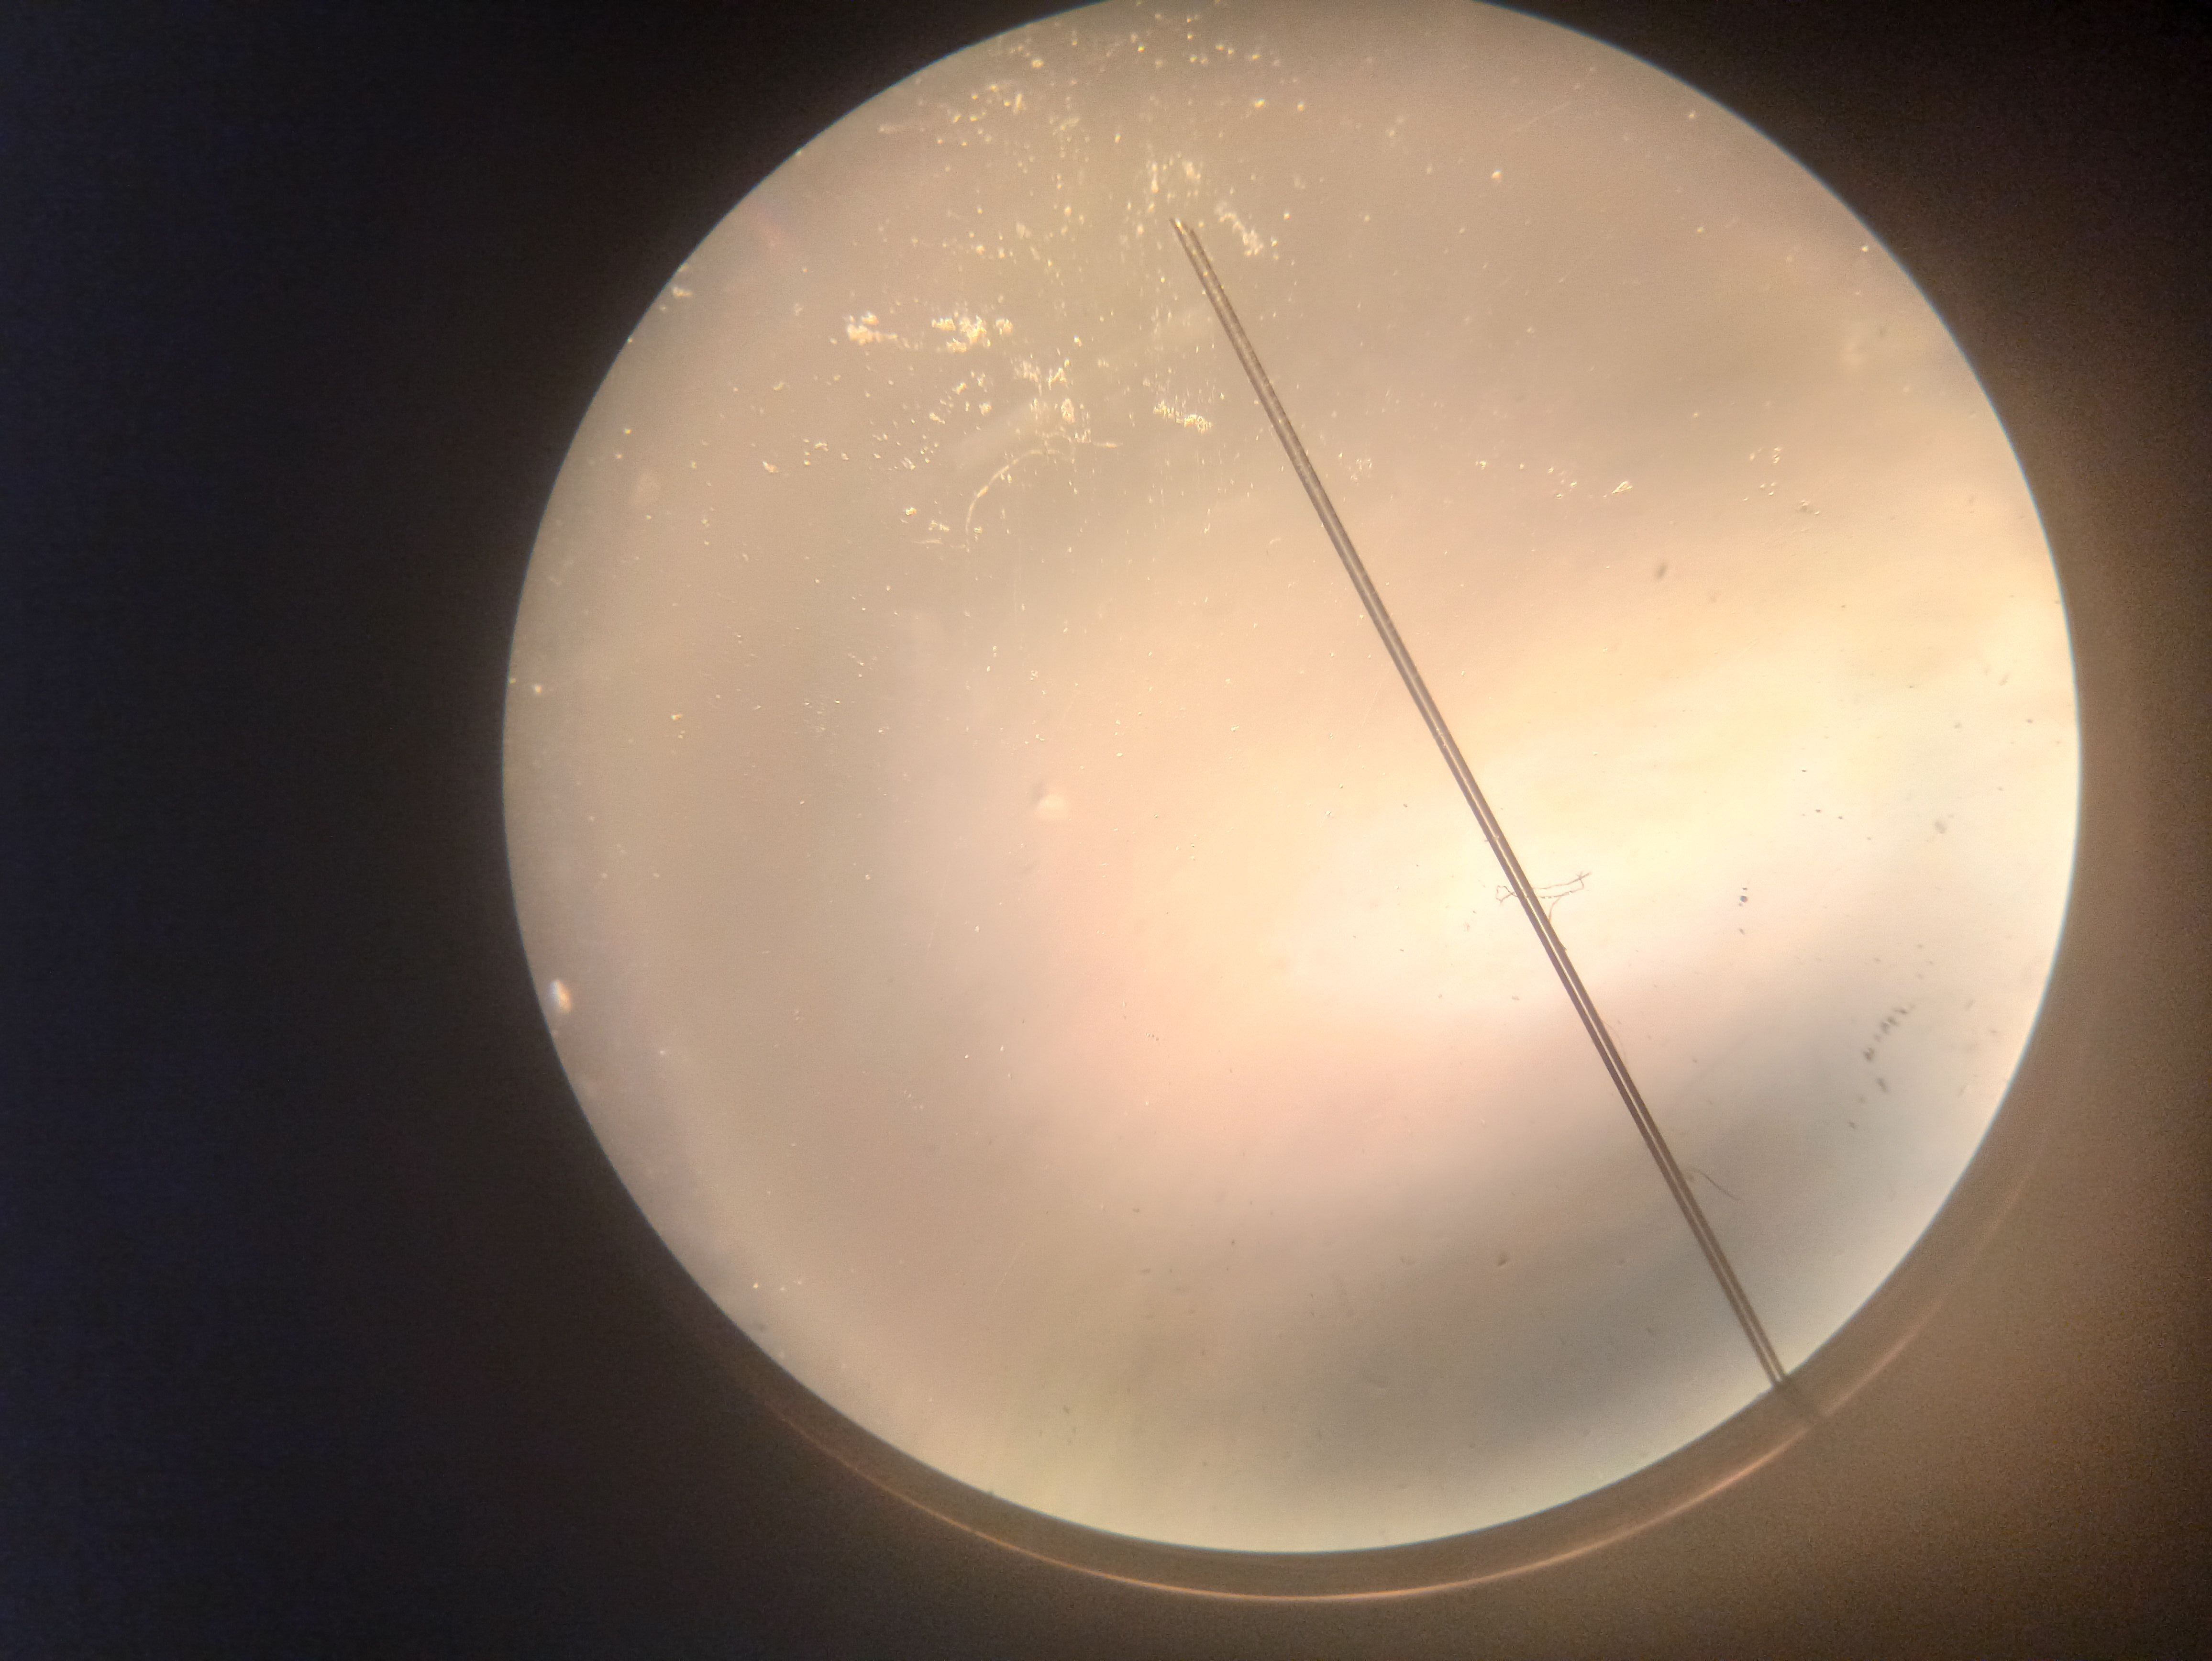
\includegraphics[width=0.6\textwidth]{text/img/odizolovano.jpg}
    \caption{\label{fig:odizolovano} Pohled mikroskopem na očištěné vlákno zbavené izolace}
  \end{figure}
  
  \subsection{Lámačka s diamantovým kotoučem}
    Vlákno zbavené ochrany bylo vloženo do lámačky a zlomeno.
    Následně bylo opět vloženo pod mikroskop, výsledek je viditelný na obrazcích \ref{fig:diamKot} a \ref{fig:diamKot_O}
    Jak je vidět, výsledný lom nedosahuje dostatečné kvality pro optický spoj, a ani po opakovaném pokusu se výsledek znatelně nezlepšil.  

    \begin{figure}[h!]
      \centering
      \includegraphics[width=0.6\textwidth]{text/img/diamantovyKotouc.jpg} 
      \caption{\label{fig:diamKot} Pohled mikroskopem na vlákno zlomené diamantovým kotoučem}
    \end{figure}

    \begin{figure}[h!]
      \centering
      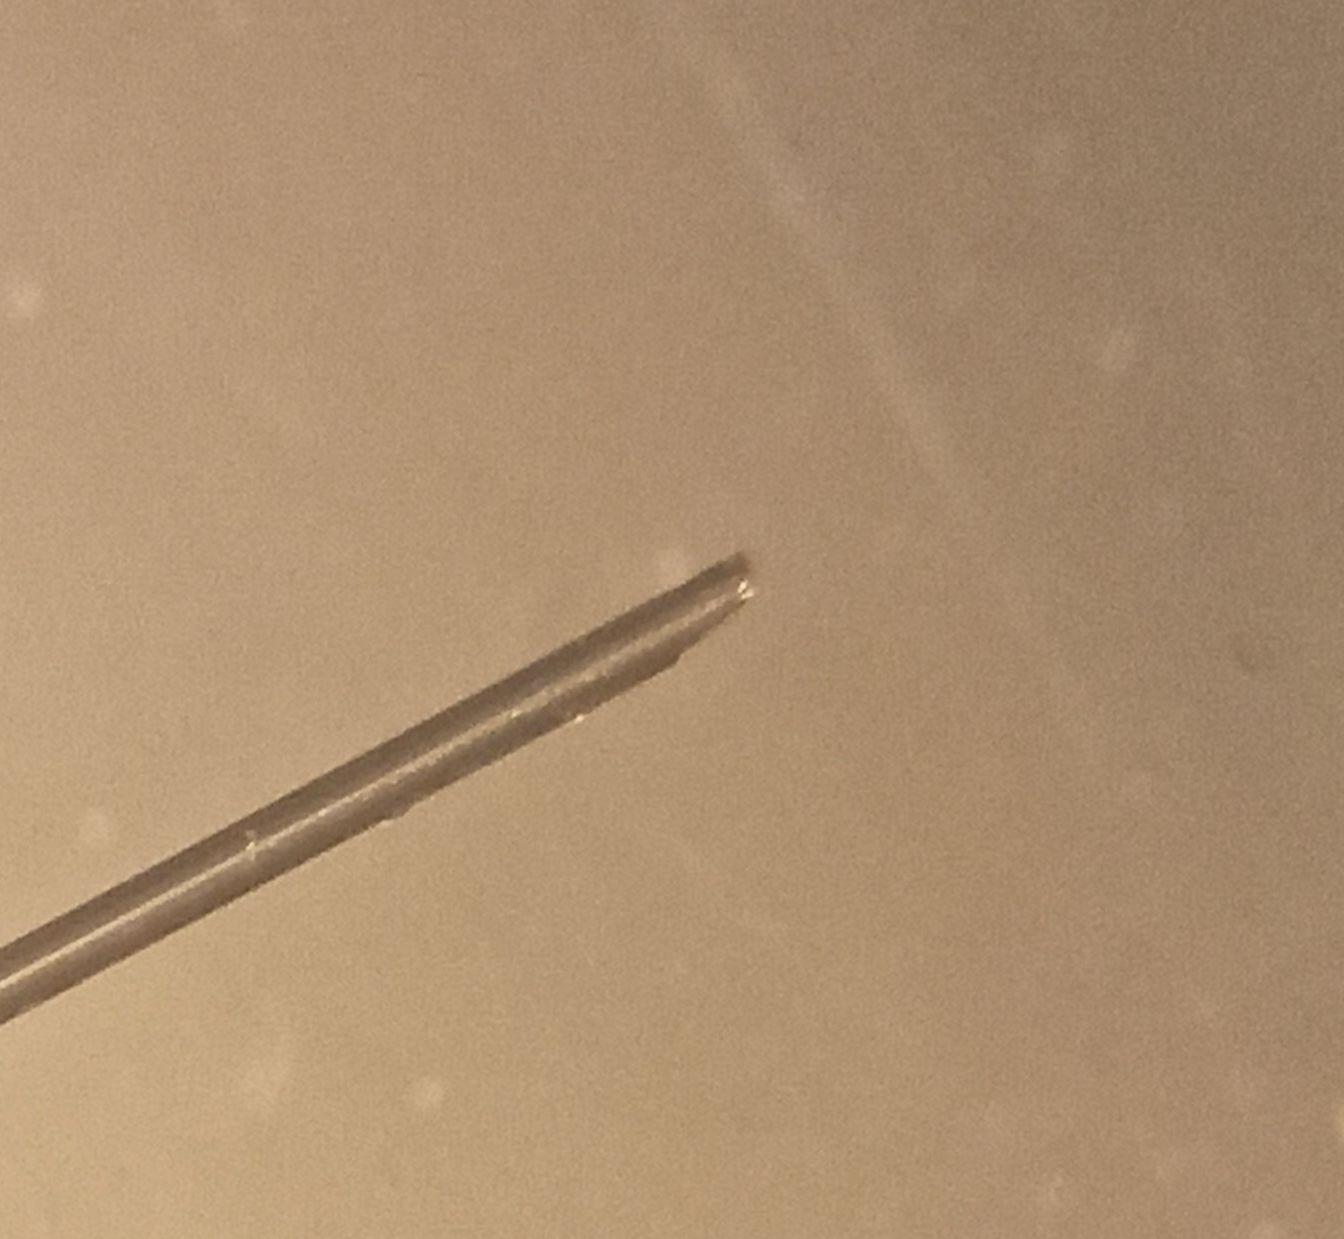
\includegraphics[width=0.6\textwidth]{text/img/diamantovyKotouc-O.jpg}
      \caption{\label{fig:diamKot_O} Oříznutý pohled na vlákno zlomené diamantovým kotoučem}
    \end{figure}

  \newpage
  \clearpage

  \subsection{Lámačka s diamantovým nožem}
    Obdobný postup byl aplikován u lámačky s diamantovým nožem.

    \begin{figure}[h!]
      \centering
      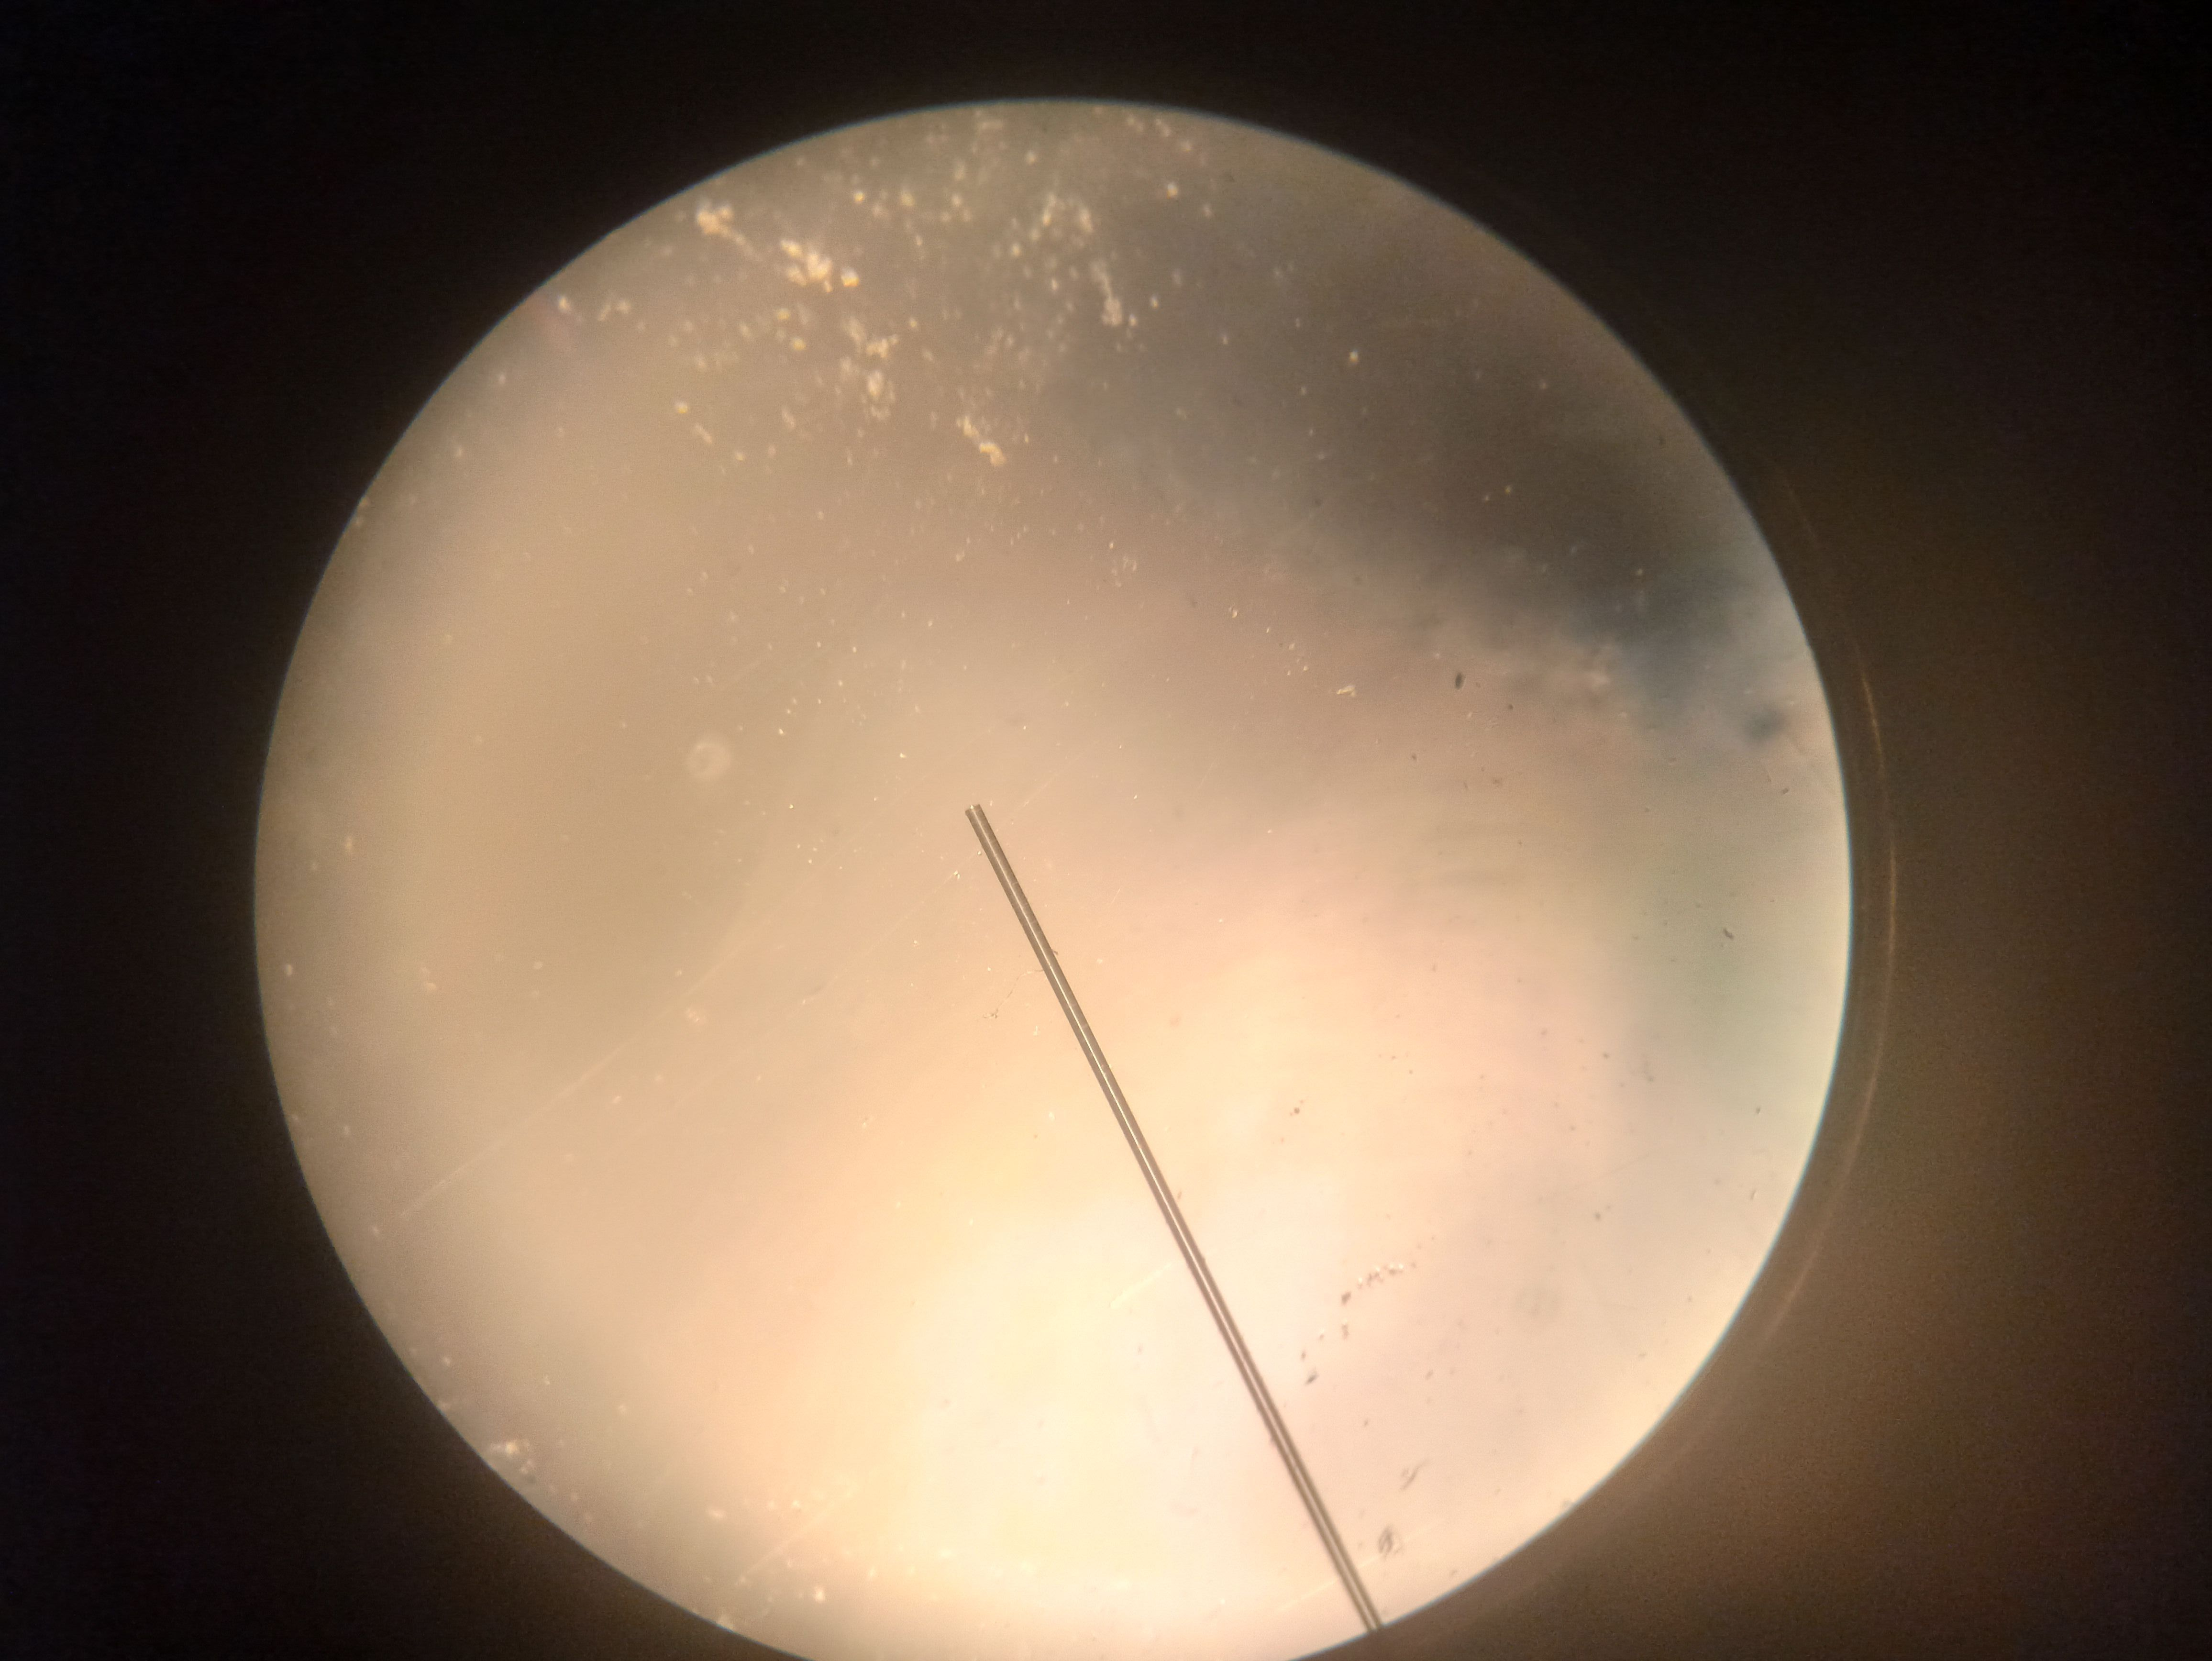
\includegraphics[width=0.6\textwidth]{text/img/diamantovyNuz.jpg} 
      \caption{\label{fig:diamNuz} Pohled mikroskopem na vlákno zlomené diamantovým nožem}
    \end{figure}

    \begin{figure}[h!]
      \centering
      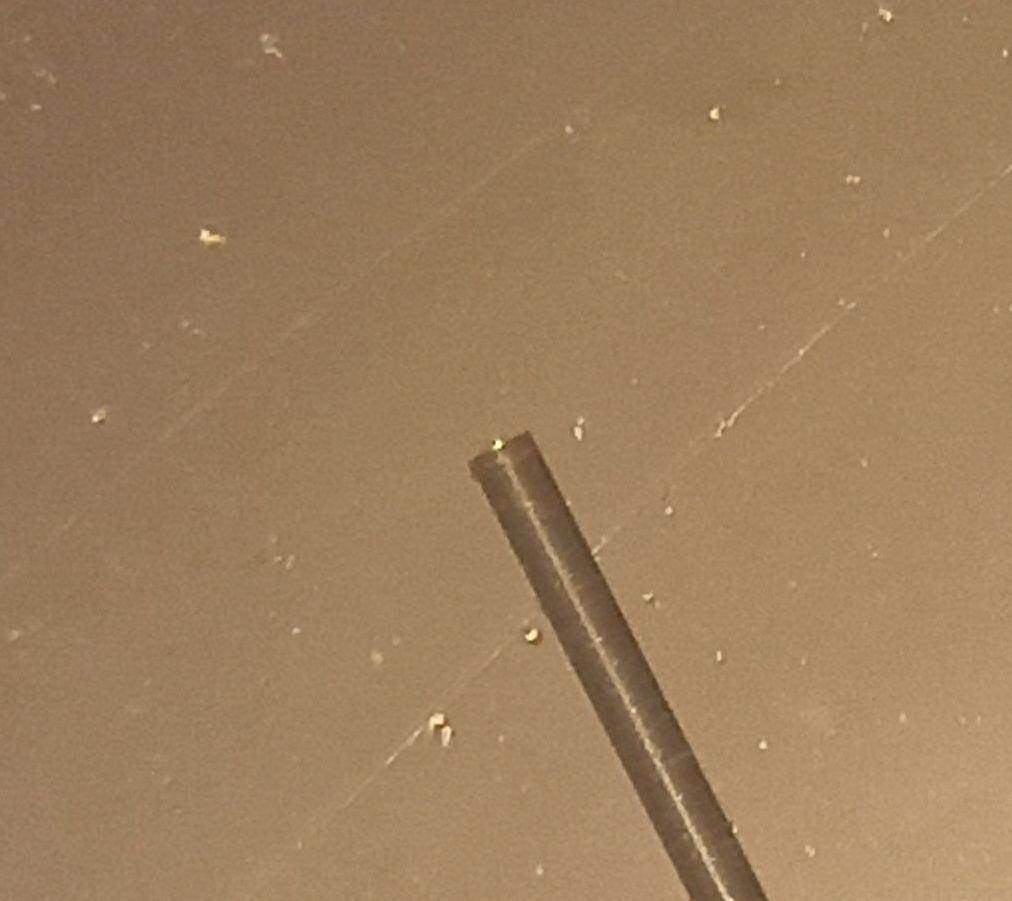
\includegraphics[width=0.6\textwidth]{text/img/diamantovyNuz-O.jpg}
      \caption{\label{fig:diamNuz-O} Oříznutý pohled na vlákno zlomené diamantovým nožem}
    \end{figure}

  \newpage
  \clearpage
  
  \vspace{-3mm}
  
  \subsection{Lom se safírovým nožem}
  
  \vspace{-3mm}

  \begin{figure}[h!]
    \centering
    \includegraphics[width=0.58\textwidth]{text/img/safirovyNuz.jpg} 
    \caption{\label{fig:safirNuz} Pohled mikroskopem na vlákno zlomené safírovým nožem}
  \end{figure}

  \vspace{-3mm}

  \subsection{Lom se safírovou destičkou}
    \vspace{-3mm}
    \begin{figure}[h!]
      \centering
      \includegraphics[width=0.58\textwidth]{text/img/safirovaDesticka2.jpg} 
      \caption{\label{fig:safirNuz} Pohled mikroskopem na vlákno zlomené safírovou destičkou}
    \end{figure}
  
  \vspace{-3mm}

  \section{Závěr}
  Jednotlivé metody lámání měly různé výsledky.
  Nejlépe se mi osvědčil diamantový nůž, který jako jediný vytvořil rovný kolmý řez.
  Nakontaktování se mi však nepodařilo vůbec. Signál procházející skrz spoj nebyl rozeznatelný od šumu, celý světelný výkon se tedy ztratil ve "spoji".

\chapter{Měření útlumu multimodového vlákna a spojek}
  \section{Zadání}
Změřte útlum optického multimodového kabelu pro vlnové délky \(1300\) a \(850~nm\). Měřte jednotlivé úseky kabelu pomocí kabelových vláknových spojek a na
závěr odvoďte ze změřených hodnot jednotkový útlum vlákna a spojky. 

\section{Měření}

\begin{table}[h]
    \centering
    \begin{tabular}{|c|c|}
        \hline
        \textbf{REF}     & \textbf{dBm} \\ \hline
        $\lambda = 850$  & -22.35       \\ \hline
        $\lambda = 1300$ & -34.39       \\ \hline
    \end{tabular}
    \caption{Referenční přenášený výkon}
\end{table}

\begin{table}[h]
    \centering
    \begin{tabular}{|c|c|c|c|}
        \hline
        1 & 2 & 3 & 4 \\ \hline
        5 & 6 & 7 & 8 \\ \hline
    \end{tabular}
    \caption{Označení vývodů}
\end{table}

\begin{table}[h]
    \centering
    \begin{tabular}{|c|c|c|}
        \hline
        \textbf{kabel}  & \multicolumn{2}{c|}{\textbf{Přenos [dB]}}                 \\ \hline
                        & $\lambda = 850$                   & $\lambda = 1300$      \\ \hline
        1               & -9.74                             & -3.28                 \\ \hline
        2               & -9.18                             & -0.50                 \\ \hline
        3               & -9.11                             & -0.46                 \\ \hline
        4               & -8.99                             & -0.43                 \\ \hline
        5               & -9.57                             & -0.28                 \\ \hline
        6               & -10.41                            & -2.16                 \\ \hline
        7               & -54.62                            & -46.94                \\ \hline
        8               & -23.10                            & -14.23                \\ \hline
        Průměr          & -16.84	                        & -8.758                \\ \hline
        Průměr 2        & -11.443 	                        & -3.303                \\ \hline
    \end{tabular}
    \caption{Útlumy různých kabelů při dvou vlnových délkách (po odečtení reference)}
\end{table}
Předpokládám, že kabel \(7\) měl nějaký problém a proto jsem přidal i řádek {\it průměr 2}, ze kterého jsem kabel 7 vyřadil.



\chapter{Měření vláknového děliče světla a vláknového cirkulátoru}
  \section{Zadání}

\begin{enumerate}
    \item Zjistěte dělící poměr vláknového děliče světla (splitteru).
    \item Ověřte funkci vláknového cirkulátoru. Přiřaďte jednotlivým číslům (portům) cirkulátoru barvy optických vláken z obr. 2 dle měřeného cirkulátoru. 
\end{enumerate}

\section{Měření}

\begin{table}[h]
    \centering
    \begin{tabular}{|l|c|c|c|}
        \hline
        & \multicolumn{3}{c|}{útlum \([dB]\)} \\ \hline
        dělička                      & 1    & 2   & 3   \\ \hline
        vstup $\rightarrow$ výstup1  & 13.3 & 5.1 & 5.9 \\ \hline
        vstup $\rightarrow$ výstup2  & 2.53 & 4.7 & 5.5 \\ \hline
        výstup 2 $\rightarrow$ vstup & 3.1  & 5.2 & 6   \\ \hline
        výstup 1 $\rightarrow$ vstup & 13.4 & 5.4 & 5.1 \\ \hline
    \end{tabular}
    \caption{Útlumy v jednotlivých směrech přenosu vláknového děliče světla}
\end{table}



\begin{table}[h]
    \centering
    \begin{tabular}{|l|c|}
    \hline
        směr přenosu      & útlum \([dB]\) \\ \hline
        C $\rightarrow$ B & 23.1           \\ \hline
        C $\rightarrow$ M & 5.5            \\ \hline
        B $\rightarrow$ C & v úrovni šumu  \\ \hline
        B $\rightarrow$ M & 25             \\ \hline
        M $\rightarrow$ C & 27.1           \\ \hline
        M $\rightarrow$ B & 5.3            \\ \hline
    \end{tabular}
    \caption{Útlumy mezi jednotlivými vývody cirkulátoru \label{tab-circuator}}
\end{table}

Z tabulky \ref{tab-circuator} mi vyplývá, že port {\bf C} je port {\bf 1}, port {\bf M} je port {\bf 2} a port {\bf B} je port {\bf 3}

\chapter{Měření přenosových vlastností modulu ADS 3000}
  \section{Zadání}

\begin{enumerate}
    \item Sestavte systém pro přenos dat a audiosignálu pomocí modulu ADS 3000
    \item Změřte šířku pásma přenášeného audiosignálu
    \item Ověřte funkčnost datového přenosu RS 232
    \item Vypracujte protokol 
\end{enumerate}

\section{Měření}

\begin{figure}[h!]
    \centering
    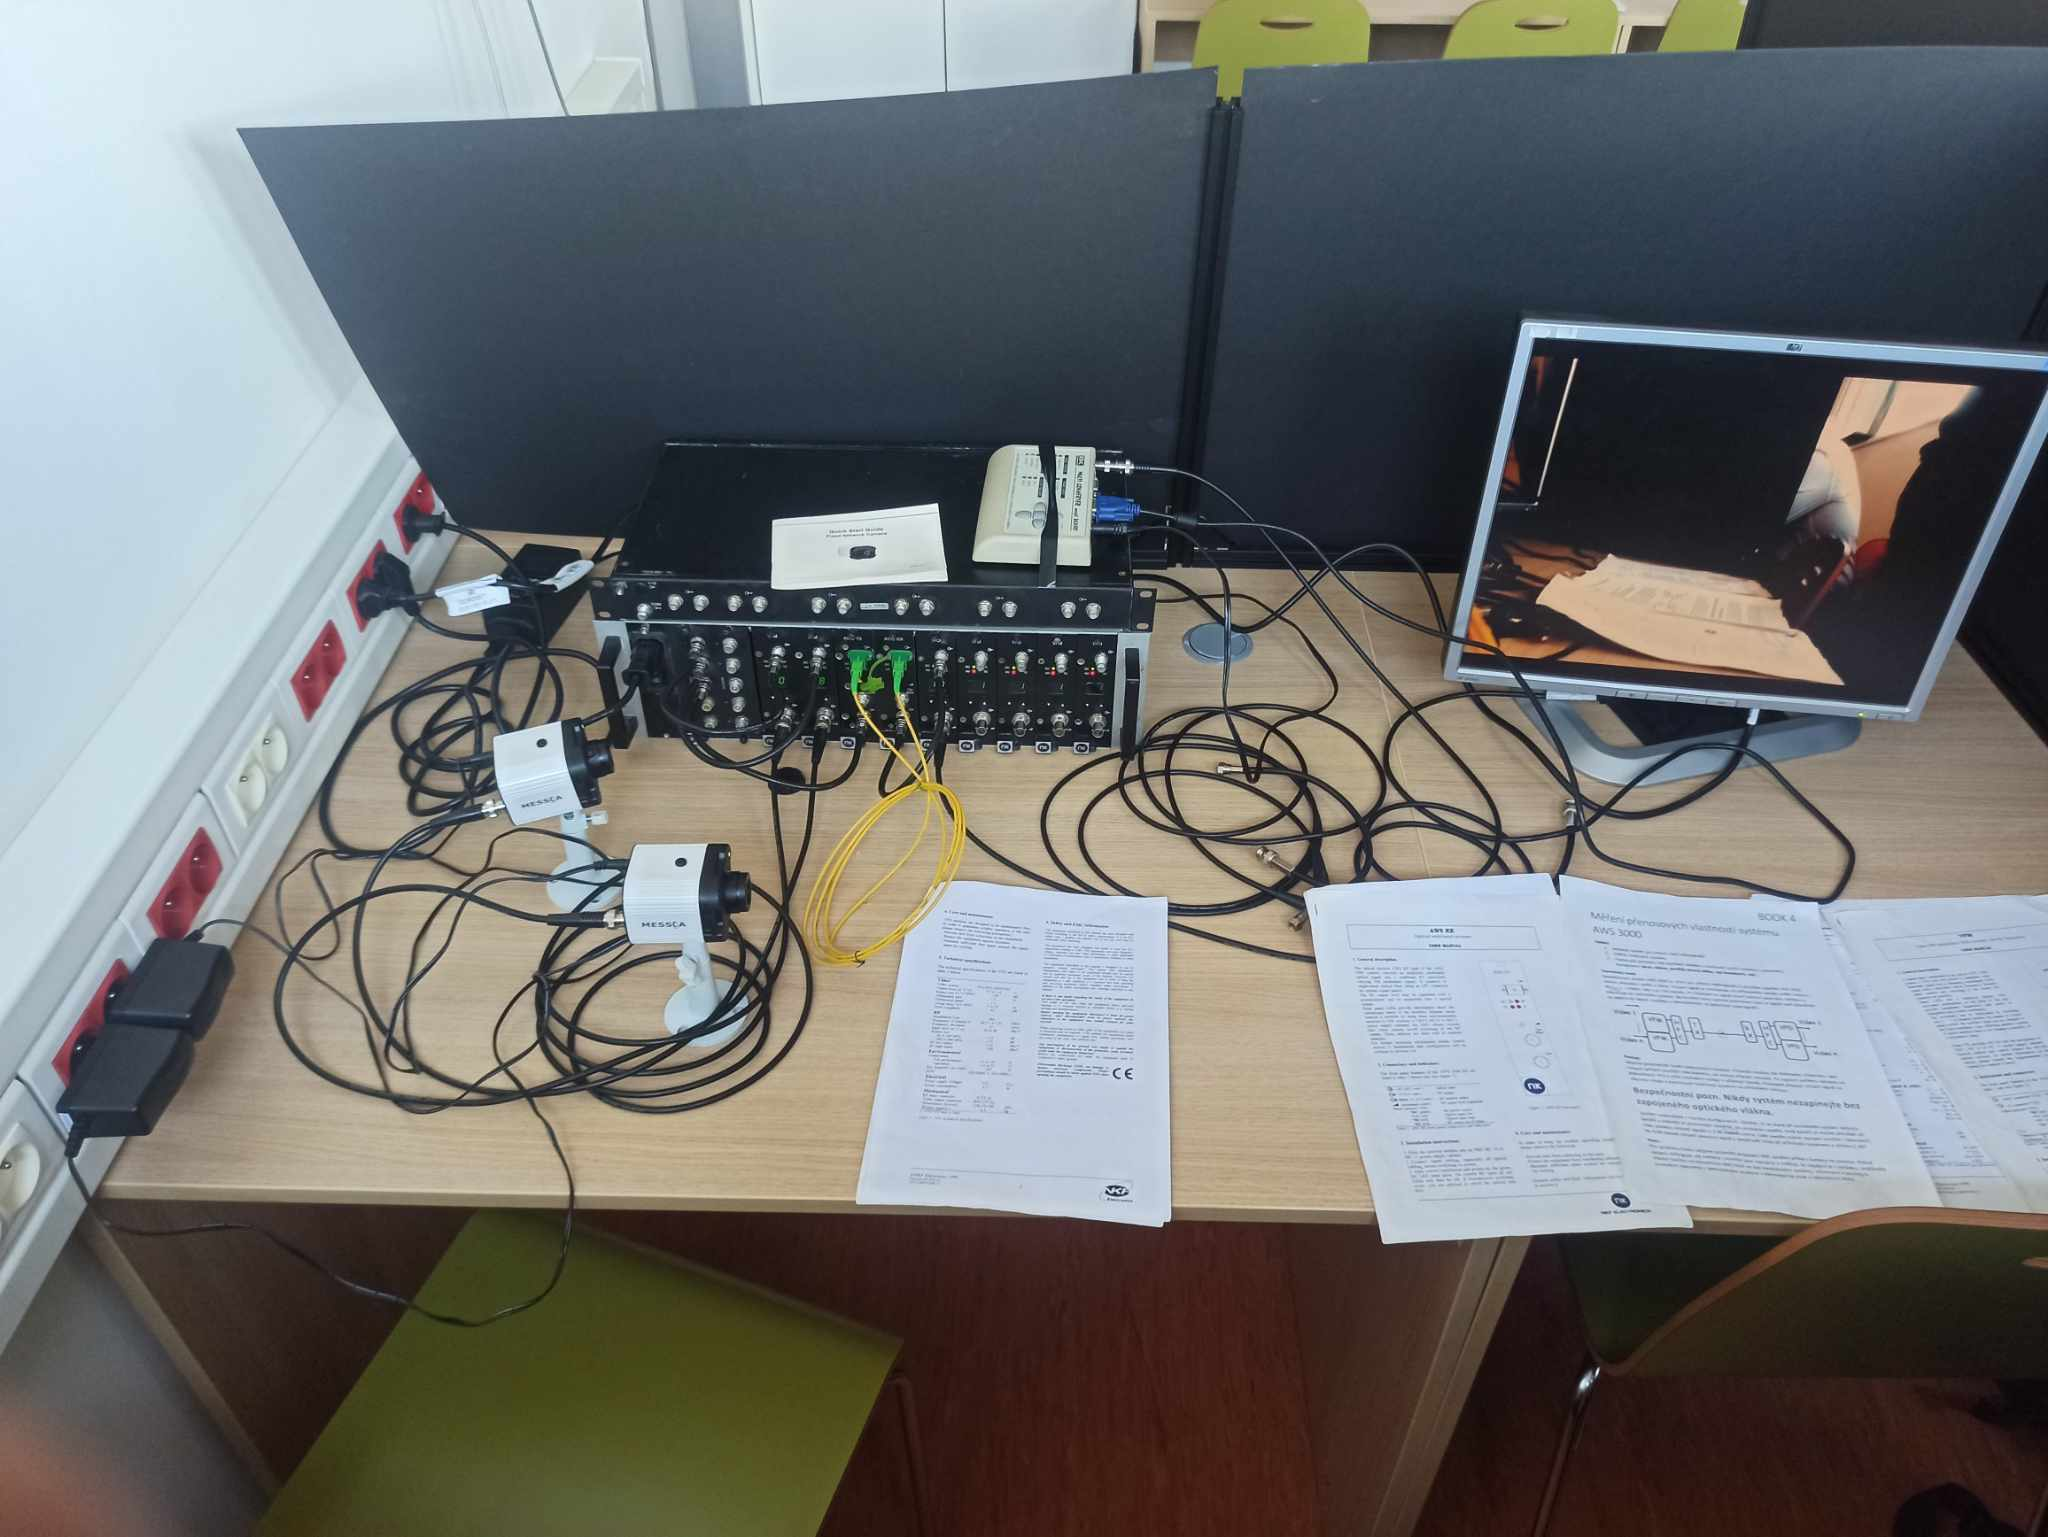
\includegraphics[width=0.58\textwidth]{text/img/ADS3000.jpg} 
    \caption{\label{fig:ADS} Sestavený systém}
\end{figure}

Audiosignál lze přenášet od \(20 [hz]\) do \(15 [kHz]\), při vyšších frekvencích dochází k nahodilému posunu fáze a k útlumu signálu.
Při nižších frekvencích dochází jen k výraznému útlumu.

RS232 lze provozovat do \(200 [kHz]\) a při vyšších frekvencích dochází k otočení fáze.
Rs232 má definovaný rozsah pro log jedničku \(3\) až \(15 [v]\) a log nulu \(-15\) až \(-3 [v]\). 
Na vstupu jsem posílal \(\pm 5\) a na výstupu četl \(\pm7\), což odpovídá standardu.




\chapter{Simulace spektrálních vlastností vláknových mřížek }
  \section{Zadání}
Nasimulujte spektrální vlastnosti vláknových mřížek. Odrazivosti jednotlivých typů mřížek
vložte do jednoho grafu a porovnejte výsledné vlastnosti. Parametry simulovaných mřížek
jsou následující: 
\begin{table}[h]
    \centering
    \small
    \begin{tabular}{|p{2.5cm}|p{3.9cm}|p{6cm}|p{3.9cm}|}
        \hline
        \textbf{Typ mřížky} & \textbf{Homogenní mřížka} & \textbf{Apodizovaná mřížka (bez kompenzace, s kompenzací $n_{eff}$)} & \textbf{Chirpovaná mřížka} \\ \hline
        Délka [mm] & 30 & 30 & 10 \\ \hline
        $\Delta n$ & 3E-5 & 6E-5 & 5E-4 \\ \hline
        Chirp [nm/mm] & 0 & 0 & 0.2 \\ \hline
        Profil apodizace & Homogenní (bez apodizace) & Gaussovský (bez kompenzace, s kompenzací) & Homogenní (bez apodizace) \\ \hline
        Spektrum [nm] & 1549-1551 & 1549-1551 & 1544-1556 \\ \hline
    \end{tabular}
    \caption{Porovnání mřížek}
    \normalsize
\end{table}

Pro všechny mřížky zvolte parametry vlákna: \(nc = 1.4488\), \(ncl = 1.44402\), \(d = 9.6 [\mu m]\). 
Všechny simulace provádějte pro rezonanční vlnovou délku \(1550 [nm]\). 
Počet sekcí volte tak, aby vycházela přibližně 1 sekce na \(50 [\mu m]\) délky mřížky.
Dále zjistěte, jak následující parametry mění výsledné spektrální vlastnosti mřížky: délka, změna indexu lomu \(\delta n\), tvar periody, hustota vzorkování.
Z grafů odečtěte šířku odraženého pásma při poklesu o \(3 [dB]\), maximální odrazivost v \% a potlačení postranních pásem oproti hlavnímu maximu v \(dB\). 
Pro lineárně chirpovanou mřížku určete také směrnici grupového zpoždění. 

\newpage

\section{Simulace}

\begin{figure}[h!]
    \centering
    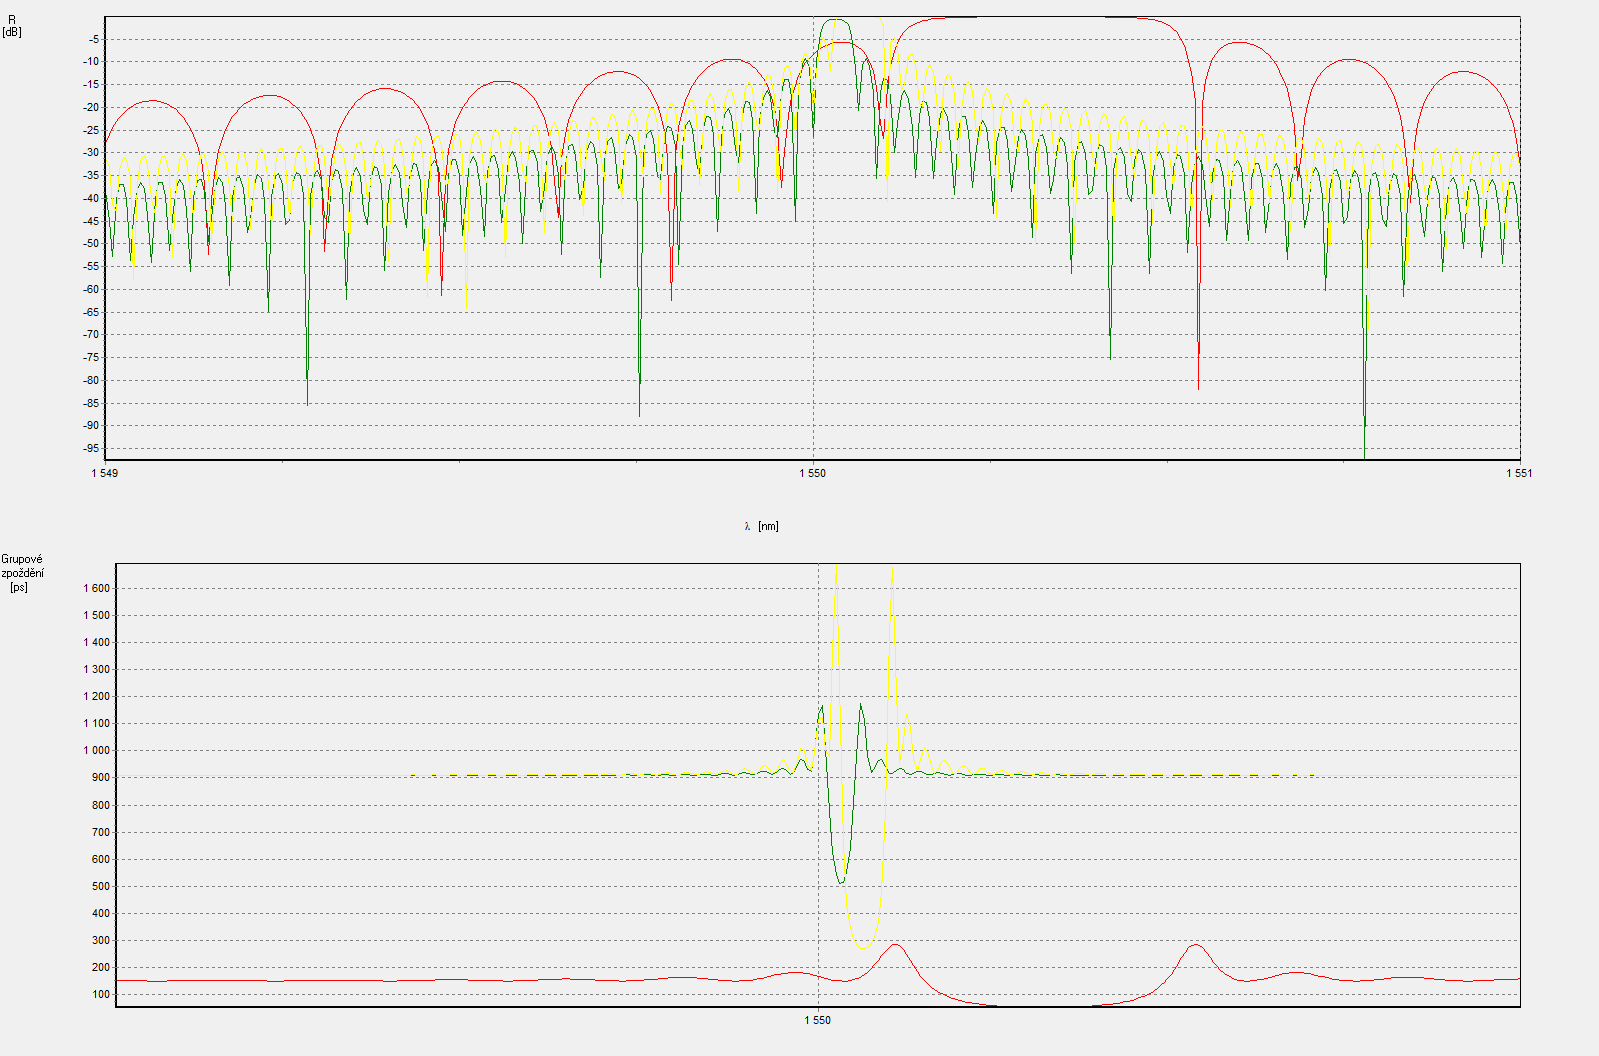
\includegraphics[width=\textwidth]{text/img/simulace-1.png}
    \caption{\label{fig:simulace} simulace}
\end{figure}



\chapter{Měření vlivu ohyby na útlum vlákna}
  \section{Zadání}
Změřte útlum vlákna při ohybu s poloměrem \(14\), \(18\), \(22\) a \(25 [mm]\) s různým počtem závitů.

\section{Měření}

\begin{table}[h]
    \centering
    \caption{Útlum v závislosti na průměru závitu, počtu závitů a vlnové délce}
    \begin{tabular}{|c|c|c|ccccc|}
        \hline
        průměr závitu \([mm]\) & & vlnová délka \([nm]\)    & \multicolumn{5}{c|}{útlum \([dB]\)}  \\ \hline
           & počet závitů & & 1    & 7      & 10    & 13    & 15                \\ \hline
        14 & & 1310         & 0.05 & 0.33   & 0.49  & 0.60  & 0.73              \\
        18 & & 1310         & 0.02 & 0.07   & 0.06  & 0.09  & 0.16              \\
        22 & & 1310         & 0.02 & 0.04   & 0.00  & 0.07  & 0.04              \\
        25 & & 1310         & 0.00 & 0.02   & 0.04  & 0.10  & 0.05              \\ \hline
        14 & & 1550         & 1.63 & 10.12  & 13.6  & 19.00 & 22.00             \\
        18 & & 1550         & 0.32 & 2.83   & 4.08  & 5.33  & 6.05              \\
        22 & & 1550         & 0.02 & 0.41   & 0.58  & 0.63  & 0.81              \\
        25 & & 1550         & 0.06 & 0.28   & 0.20  & 0.24  & 0.36              \\
        \hline
    \end{tabular}
\end{table}


\end{document}